\documentclass{article}
\usepackage{main}

\title{Boîtes de Pétri}
\author{}
\date{2 Février 2024}

\begin{document}
\maketitle
\begin{center}
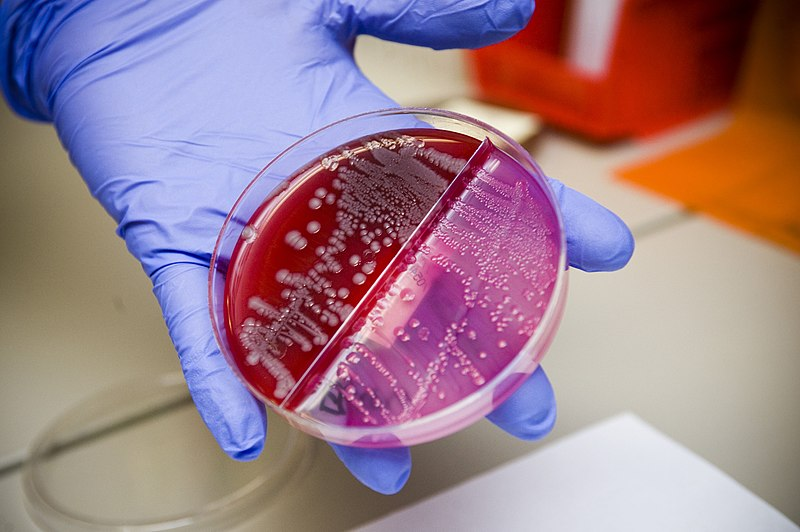
\includegraphics[scale = 0.3]{Petri.jpg}
\end{center}
Dans une boîte de Pétri, on fait grandir une population de bactéries. Chaque jour, cette population augmente de $7\%$. Mais en cas de surpopulation dans la boite de Pétri (si la population a augmenté de plus de $40\%$ par rapport à la population initiale), les bactéries meurent, et la population diminue alors de $32\%$. 
\begin{enumerate}
\item La population de bactérie a-t-elle augmentée ou diminuée au bout de 10 jours ?
\item De quel pourcentage doit-on diminuer ou augmenter la population obtenue après $10$ jours pour retrouver la population initiale ?
\end{enumerate}
\end{document}